\documentclass[12pt]{article}

\usepackage[a4paper, left=2.5cm, right=2.5cm, top=2.5cm, bottom=2.5cm]{geometry}
\usepackage{times}

\usepackage[font=small, labelfont=bf]{caption}
\usepackage[subrefformat=parens]{subcaption}

\usepackage[indent=0pt]{parskip}
\usepackage{setspace}
\onehalfspacing

\usepackage{graphics,graphicx}
\usepackage{float}
\usepackage{svg}
\graphicspath{{../Figures/}}
\usepackage{mwe}

% Maths formatting
\usepackage{amsmath}
\usepackage{braket}

\usepackage{amsthm}
\newtheorem*{theorem}{Theorem}
\theoremstyle{definition}
\newtheorem*{definition}{Definition}
\newtheorem{condition}{Condition}

\usepackage[utf8]{inputenc}
\DeclareUnicodeCharacter{2212}{$-$} % Minus sign
\DeclareUnicodeCharacter{03BC}{µ}

% Bibliography
\usepackage[backend=biber, sorting=none]{biblatex}
\addbibresource{thesis.bib}

% Number formatting
\usepackage[round-mode=figures,round-precision=3,round-pad=false,mode=text]{siunitx}

%\usepackage{multirow} % Multi-row cells in tables
%\usepackage{booktabs} % Nice table separators

% Clever references
\usepackage[hidelinks]{hyperref}
\usepackage[nameinlink,capitalise,noabbrev]{cleveref}
\crefname{condition}{Condition}{Conditions}

% Rename environments
\renewcommand{\listfigurename}{List of figures}
\renewcommand{\listtablename}{List of tables}

%\usepackage{float}

\title{\Huge \bfseries Quantum annealing\\for music arrangement}
\author{Lucas Kirby\\\normalsize Department of Physics, University of Durham\\\\\normalsize Supervised by\\\normalsize Prof Robert Potvliege \& Dr Omer Rathore}
\date{\normalsize 23 April 2025}

\begin{document}

\maketitle

\vfill

\addcontentsline{toc}{section}{Abstract}
\begin{abstract}              

Music arrangement is usually a complex and time-consuming process; this paper aims to provide an automatic method by which to arrange music via a quantum computing technique called quantum annealing. By splitting a score into a set of phrases, these phrases can form a quadratic unconstrained binary optimisation (QUBO), a function which the quantum computer aims to minimise by choosing the values of discrete variables. At the end of the optimisation process, the resulting chosen values describe the final arrangement, which can then be interpreted into sheet music. This method is tested on an excerpt of Beethoven's String Quartet No. 10 in E-flat major; in this case, the optimisation process is successful, and selects compatible phrases that produce a suitable arrangement.

\end{abstract}

\vfill

\begin{center}
    \includesvg{durham-university.svg}
\end{center}

\thispagestyle{empty}
\clearpage

\tableofcontents
%\listoffigures
%\listoftables

\thispagestyle{empty}
\clearpage

\section{Introduction}

% Background to quantum computing
The field of quantum computing has its foundations as early as the 1980s, with the suggestion that hardware following the laws of quantum mechanics could be faster and more powerful than its classical counterpart [CITE].
Quantum computers, which leverage quantum mechanical phenomena to perform calculations, store information as qubits (``quantum bits'') which can exploit effects such as superposition and entanglement to increase computing power.
With the age of quantum computing came the possibility to solve complex problems usually intractable to even the most powerful classical computers. 
Since its inception, two methods of quantum computing have been developed: gate-based computing and adiabatic quantum computing.

% Gate-based
Gate-based quantum computers use quantum gates to manipulate qubits, analogous to classical logic gates for conventional circuits, where gates can be represented as operators acting on qubit states. This kind of computer is versatile and well-suited to solving general problems, and is being actively developed by several technology companies as the next step in general computing \cite{google}\cite{ibm}.
% Quantum annealing
Adiabatic quantum computers, on the other hand, rely on the application of the adiabatic theorem to slowly evolve a quantum system. This is often used to find the global minimum of a given function which would be almost impossible to solve analytically, which often involves brute-force methods. Adiabatic quantum computers have been used to find solutions to a variety of optimisation problems, such as protein folding \cite{perdomo-ortiz_protein_2012}, financial portfolios \cite{phillipson_portfolio_2021}, and traffic flow \cite{inoue_traffic_2021}.

At time of writing, quantum computing is still a nascient field, with quantum computers remaining impractical for real-world applications. In theory, larger and more advanced quantum computers would be able to solve problems in much shorter timeframes than classical computers, an advantage dubbed ``quantum supremacy''. The achievement of this would trigger an upheaval of many common computer systems, most importantly encryption and simulation [CITE]. A recent study has claimed to demonstrate this advantage using adiabatic quantum computing to analyse the structure of magnetic materials [CITE], although this is a specialised application and far from demonstrating an overall ``supremacy'' over classical methods.

% Computer music
The combination of computing and music is a relatively new field, with the involvement of quantum computers even more so. Music is often seen as a very human endeavour, where only skilled musicians could compose and perform such sequences of sound that would be considered art. The idea that computers could produce music arose as early as the 19th century, with the conception of the first general-purpose computer, the Analytical Engine\footnote{The computer was never actually built, but laid the foundation for many modern computing concepts.} [CITE], with Ada Lovelace, considered the first computer programmer, noting that ``the engine might compose elaborate and scientific pieces of music of any degree
of complexity or extent''. The first computer composition would not be produced until nearly a century later [CITE], and since then various approaches to computer music have been taken, ranging from fractals [CITE], Markov chains [CITE], and evolutionary models [CITE]. Quantum computing is the latest iteration of computer music, opening up new and unique possibilities.

% Quantum computer music
Since its emergence into the computer music scene, quantum computers have been used to write melodies [CITE], develop harmonies [CITE], create synthesisers [CITE], produce variations of original scores [CITE], and create intelligent musical systems via quantum natural language processing (QNLP), using a mixture of gate-based and adiabatic methods. However, these efforts have been directed at music \emph{composition}, that is, the generation of entirely new sequences and sounds, rather than music \emph{arrangement}, the adaptation of previously-composed pieces. Indeed, at time of writing, the application of quantum computing to the problem of music arrangement has never been explored before.

% Study overview
In this study, we propose that music arrangement can be formulated as an optimisation problem to be solved using a version of adiabatic quantum computing called quantum annealing.
The structure of the study is as follows: we first introduce the relevant theory for both quantum annealing as a computational tool, and music arrangement as a suitable problem to solve; we then propose a detailed framework for combining the two, and apply this method to two musical scores; finally, we consider conclusions and possible future work.

\section{Quantum annealing}

Before we consider quantum annealing, we must first discuss adiabatic quantum computing (AQC), from which it draws its main principle. AQC is a computing technique that works under the adiabatic theorem.

\begin{theorem}[Adiabatic theorem]
    A physical system remains in its instantaneous eigenstate if a given perturbation is acting on it slowly enough and if there is a gap between the eigenvalue and the rest of the Hamiltonian's spectrum. \cite{born_beweis_1928}
    \label{thm:adiabatic}
\end{theorem}

A linear evolution of the Hamiltonian of the system can be expressed as
\begin{equation}
    H(t)=\left(1- \frac{t}{T}\right)H_0 + \frac{t}{T}H_p
    \label{eq:time-evolution}
\end{equation}
where we are evolving from an initial Hamiltonian $H_0$ to a final Hamiltonian $H_p$ over a time interval $T$. If we start in the $n$th state of $H_0$, then, given that the evolution is slow enough and that there is some energy difference between eigenstates (i.e.\ non-degenerate), $H(t)$ will remain in the $n$th instantaneous eigenstate throughout evolution and end in the $n$th state of $H_p$. How ``slow'' the evolution needs to be is determined by the minimum energy gap of the instantaneous Hamiltonians; an approximate adiabaticity criterion can be given by
\begin{equation}
    \frac{\hbar\braket{\psi_m|\dot{H}|\psi_n}}{(E_n-E_m)^2} \ll 1
    \label{eq:energy-gap}
\end{equation}
where we have used the largest matrix element between a pair of eigenstates $\psi_{n,m}$, and ${E_n-E_m}$ is the minimum energy gap. It can be seen that a smaller energy gap requires a slower evolution in order to remain adiabatic, and that for degenerate energies ($\Delta E=0$) no adiabatic evolution is possible. 

This technique is useful as it allows particular eigenstates (usually the ground state) of a very complicated Hamiltonian ($H_p$) to be found simply by evolving from a Hamiltonian whose eigenstate is easy to find and prepare ($H_0$). Importantly, this process is universal and deterministic---if the system starts in the ground state of $H_0$, then it is guaranteed to be in the ground state of $H_p$ after evolution.

However, since a truly adiabatic process takes infinitely many steps and therefore an infinite amount of time, this is not possible in practice. Instead, the adiabaticity condition of AQC can be relaxed to allow a shortening of the evolution time---this is quantum annealing\footnote{In metallurgical terms, annealing is the process of heating and cooling a material to alter its physical properties. Much like its metallurgical counterpart, quantum annealing allows a system to settle into a more useful final state.}. Over these shortened timescales ($T\sim\unit{\us}$), the process is now heuristic and the eigenstate after evolution is no longer guaranteed, but follows a probability distribution. The advantage of this method is that a particular evolution can be run many times, sampling the distribution of final states until an acceptable outcome is found.

The main use of quantum annealing is to solve combinatorial optimisation problems, which are problems that require the minimisation of a function over a discrete set of variables. If $H_p$ is prepared such that its ground state encodes the solution to the optimisation problem, then as long as the initial Hamiltonian is prepared in the ground state, the solution is likely to be given at the end of the annealing process. In the field of computational complexity, these problems belong to a class of complex problems called NP (nondeterministic polynomial-time). A full discussion of computational complexity is beyond the scope of this study, but in brief NP problems are difficult to solve via classical algorithms as the time to solution scales exponentially with problem size (hence nondeterministic). Problems like these have large solution spaces with many local minima, which cannot be solved quickly. A common example is the travelling salesman problem: a salesman must visit a set of cities exactly once and return home, whilst minimising the distance travelled [CHECK THIS]. As the number of cities increases, the number of possible routes the salesman could take grows exponentially, with a classical algorithm having to consider many more possible options. It is these sorts of optimisation problems that quantum annealers excel at solving.

In order to encode a problem, problem Hamiltonians ($H_p$) take the form of an Ising spin glass, a random arrangement of magnetic dipole moments (discrete variables) that can be in one of two states, typically spin-up ($+1$) or spin-down ($-1$) [CHECK THIS]. A spin glass with a vector $s$ of $N$ spins takes the form
\begin{equation}
    H(s) = \sum_{i<j}^{N}J_{ij}s_i s_j + \sum_{i=1}^{N}h_i s_i
    \label{eq:ising}
\end{equation}
where $J_{ij}$ are the coupling strengths between spins, and $h_i$ are the field strengths of individual spins. The quantum equivalent can be expressed as
\begin{equation}
    H_p = H(\sigma^z)
\end{equation}
where we have replaced the spins with Pauli matrices. This is the Ising model, with the discrete variables now \emph{qubits}---binary variables like their classical counterparts, but existing in a superposition of the two states until measurement. The corresponding ground state is prepared with the Hamiltonian
\begin{equation}
    H_0 = h_0\sum_{i=1}^{N}\sigma_i^x
\end{equation}
which is an equal superposition of all possible states in the eigenbasis of $H_p$ [CHECK THIS].

Another way of expressing problems is via the QUBO (quadratic unconstrained binary optimisation) model. A QUBO model takes the form of a function $f(x)$ to be minimised, and takes the form
\begin{equation}
    f(x)=\sum^N_{i<j}Q_{i,j}x_ix_j + \sum^N_{i=1}Q_{i,i}x_i
    \label{eq:qubo}
\end{equation}
where $x\in[0,1]$ is a new vector of binary variables, and $Q$ is an $N\times N$ upper-diagonal matrix of real weights. The off-diagonal $Q_{i,j}$ terms are known as quadratic coefficients, and diagonal $Q_{i,i}$ terms as linear coefficients. These two models are mathematically equivalent, and each can be transformed to the other via a change of variable
\begin{equation}
    s_i = 2x_i - 1 \,.
    \label{eq:qubo-ising}
\end{equation}
Whilst there are merits for each model, this study exclusively uses QUBO models to express optimisation problems.

\subsection{Quantum hardware}

% Should be near reference
\begin{figure}[h]
    \centering
    \includesvg[width=0.5\linewidth]{../Figures/pegasus.svg}
    \caption[A graph of \num{144} qubits in a D-Wave QPU.]{A graph of \num{144} qubits in a D-Wave QPU, using their Pegasus topology. Qubits are represented by vertices, and couplers by edges.}
    \label{fig:pegasus}
\end{figure}

Once a problem has been expressed with an Ising or QUBO model, it is sent to a quantum processing unit (QPU) to be solved. These units takes the form of a physical Ising spin glass, a lattice of physical qubits connected via couplers. The qubit biases and coupling values are influenced by electromagnetic fields, allowing the mapping of models to physical qubits, with linear terms as qubits and quadratic terms as couplers between them. This mapping process is known as \emph{minor embedding}, and is often handled by a classical computer `on the fly' each time a problem is submitted, introducing a slight computational overhead to running a problem. Fixed embeddings can be specified, but these require \textit{a priori} knowledge of the specific QPU architecture. Once embedded, the system can be prepared in its initial ground state, and allowed to evolve to its final state to obtain the solution.

Often, the topology of a QPU doesn't allow an exact one-to-one mapping of a problem to physical qubits. It may be the case that the problem requires a variable to have a higher degree (number of connections) than the number of couplers physically allowed by the QPU. The solution to this is the introduction of chains---connected physical qubits chained together, acting like a single discrete variable, which enables the necessary mapping. The chain strength determines how strongly the chain is coupled, enforcing that all qubits within the chain to have the same value in order for it to remain discrete. Chain strength is an important parameter that can affect the quality of solutions, and can be tuned. If it is too weak, a final state may include chain breaks: chains where the interconnected qubits differ in value. Conflicts like these can be solved via different approaches, a common one being majority vote, which sets the value of the corresponding discrete variable to the modal value of the chain. However, since this operation is done by a classical computer after the annealing process, the switch may result in an undesirable, sub-optimal solution, and so chain breaks are often best avoided. Alternatively, if the chain strength is too strong, it can overpower the other terms in the problem model, resulting in poor optimisation.

QPU annealers (also known as solvers) have many other parameters that can be tuned, influencing exactly how the annealing process is carried out and significantly affecting the quality of solutions [CITE SOLVER WEBSITE]. Aside from chain strength, others that this study considers are anneal time per sample and number of reads. Both these parameters affect the total QPU access time, and so finding a balance between them is key to minimising the time to solution.

As mentioned previously, the time interval for each sample (evolution) is short in order to relax the adiabatic condition. For simple problems this is sufficient to return optimal solutions with a high likelihood, however, as the problem size increases this may no longer be the case. For a problem with $N$ qubits there are $2^N$ energy levels, with the relative size of spectral gaps (differences between energy levels) decreasing with $N$ [ASK ABOUT THIS]. As seen in \cref{eq:energy-gap}, smaller spectral gaps ($\Delta E$) require longer anneal times ($T$) to prevent excitation to higher energy states, such that the uncertainty in energy eigenstate is not large enough to eclipse this gap. (minimum energy gap?) The exact time evolution during this interval can also be customised to control results further \cite{khezri_customized_2022}, although this is beyond the scope of this study.

A benefit of shortened anneal times is that the system can be evolved and measured (sampled) many times, increasing the likelihood that a lower-energy solution from the distribution will be found. An evolution sampled many times creates a distribution in solution energy: for a simple QUBO model with a sparse matrix $Q$, this distribution may be biased towards lower energies therefore needing fewer samples; for a complicated matrix with many entries, the sampled distribution tends towards a Gaussian [RANDOM MATRIX LIT], with many more reads necessary to be likely to sample from the tail end. The density of a problem matrix can be found from a QUBO model of the form of \cref{eq:qubo} as
\begin{equation}
    \rho=\frac{V+E}{V^2}
\end{equation}
where we have defined a new graph $Q=(V,E)$, with $V$ as the number of linear coefficients and $E$ the number of quadratic coefficients. $\rho=1$ indicates a fully-connected problem, the worst-case scenario.

% D-Wave
Many companies provide both personal and commercial access to gate-based quantum computers, however, few develop the hardware necessary for quantum annealing. D-Wave Systems was the first to realise a true quantum annealer, and have since developed and released their technology to the wider scientific community. All problems in this study were submitted to D-Wave's Advantage System 4.1 solver, which boasts a topology of over qubits each with a degree of. held at cryogenic temperatures and low-magnetic field environments to prevent unwanted fluctuations.

D-Wave Systems operates the first and only quantum annealer for commercial access, introduced in 2011 . All problems in this paper are run on the D-Wave Advantage quantum system\footnote{Access kindly granted by the Durham University Physics Department.}, which uses their Pegasus architecture, an example of which can be seen in \cref{fig:pegasus}. A full Advantage QPU contains over \num{5000} qubits, each with a maximum degree of \num{15}.
Interaction with the D-Wave QPUs is handled through their Leap quantum cloud service, which is used to submit problems to solvers. D-Wave provides an open-source software development package (SDK) of Python tools which allows users to translate problems into binary optimisation and create problem models for the QPU to solve.

Quantum annealing has already been applied to a widge array of optimisation problems, ranging from financial portfolios, protein folding, and traffic flow. This study explores a creative novel application of this technique, music arrangement.

!!!Nick Chansellor paper, why quantum annealing?

\section{Music arrangement}
\label{sec:arrangement}

The first evidence of humans writing music is theorised to have originated as early as 2000BC [CITE]; since then, it has become a hallmark of the human experience, so much so that the \emph{Voyager I} probe carries over 50 tracks of music from across the world as a message to potential extraterrestrial life [CITE]. Whilst some musicians would compose entirely new music, others would build upon and adapt previously composed pieces for practical or artistic reasons, whether that be in terms of instrumentation, medium, or style, to create an \emph{arrangement}. One of the most famous examples of this is \textit{Pictures at an Exhibition}, a piano suite written by Modest Mussorgsky, but more commonly known for its orchestral arrangement by Maurice Ravel.
Traditionally, the arrangement of music is a complex process that requires a deep understanding of musical theory, structure, and style. Composers use their creativity and intuition to create a piece that is both musically interesting and emotionally engaging whilst still remaining faithful to the source material—a challenging and often time-consuming process. Perhaps it is unsurprising, then, that there has been interest in automating this process.

One of the earliest examples of this can be seen in the \textit{Musikalisches Würfelspiel} (``musical dice game'') system popular in the 18th century. The roll of dice would determine the order of pre-composed musical phrases, allowing for the creation of new music without the need for a composer. This system was engaged by the likes of Bach and Mozart, although fell out of fashion the following century.
The introduction of computers in the 20th century allowed for more sophisticated methods of music arrangement. Composers could now transpose and manipulate musical parts digitally, without the need to transcribe parts by hand. Moving into the 21st century, more advanced techniques such as genetic algorithms and neural networks have been used to arrange music, with varying degrees of success. However, these methods are limited by the complexity of the problem and the need for extensive training data.

Music arrangement refers to the art of rewriting a musical score in a new setting, style, or structure, whilst still maintaining the essence of the original. A classical example of this is Mussorgsky's \emph{Pictures at an Exhibition}, which is well known for its orchestral arrangement by Ravel but was originally a piano solo. A more contemporary example would be ???'s rendition of \emph{The Star-Spangled Banner} at the ??? Super Bowl, which caused much controversy due to its laid-back style during a time of conflict in Cuba? The rearrangement of a piece can have a great effect on how the listener interprets it, and doing this effectively is still a pertinent issue many musicians face.

Traditionally, it's a time-consuming blah blah blah. However, in this study we aim to formulate music arrangement as an optimisation problem, which can be solved like any other via quantum annealing. It has been shown that music arrangement can be reduced to an NP-hard problem \cite{moses_computational_2016}, by considering the special case of music \emph{reduction}. Reduction is a form of arrangement whereby the number of instrument parts only gets smaller, and we define here subject to the following conditions:

\begin{condition}[Uncreative]
    All music in the arrangement must come from the original, in the same order.
    \label{con:uncreative}
\end{condition}
\begin{condition}[Non-degenerate]
    Music played in one arrangement part cannot be played in another.
    \label{con:non-degenerate}
\end{condition}
\begin{condition}[Monophonic]
    Each part in the arrangement can only contain music from a single part in the original at any time.
    \label{con:monophonic}
\end{condition}

Holistically, reduction aims to fit as much original music into the parts of the arrangement, whilst still being playable. Notably, these constraints forgo the need to compose new music, a very subjective endeavour that is not handled well by optimisation.

The beginning of any arrangement process is an original musical score. There exist a myriad of musical styles, genres, instruments, and notations, each as expressive and meaningful as the next. To maintain a manageable scope, this study focuses on European Classical-era (?) small ensemble and orchestral music, written in standard Western notation. A brief taxonomy of a typical score is as follows: a standard score is split up into parts, which can be played by a single instrument or an instrument section. Each part is further divided into bars (sometimes known as measures) which contain the notes that the instrument plays. If an instrument plays more than one note at a time, it is known as polyphonic (otherwise monophonic).

...continuation of tradition.

% Theory, anyone could apply these steps. Then talk about practicalities in results (or in code appendix)
\section{Proposed framework}

Previous approaches to the automatic arrangement of music have relied on classical methods such as neural networks  or recursive classical algorithms in order to produce arrangements that are musically sound. However, these methods are limited by the complexity of the problem and the need for extensive training data. In this study, a new approach to the automatic arrangement of music is proposed by applying quantum annealing.

It has been shown that the arrangement of music can be formulated as a combinatorial optimisation problem \cite{moses_computational_2016}: given a set of musical phrases, each phrase can be assigned a binary variable and formulated into a Boolean satisfiability (SAT) problem, with variables assigned to clauses according to their compatibility. A valid solution would be an assignment of values such that the Boolean expression is satisfied, corresponding to the phrases included in the final arrangement . Phrases are chosen as the smallest unit of music instead of notes to best preserve important melodic lines and harmonies, which may sound dissonant or confusing if split up.


We propose a new framework for the arrangement of music via quantum annealing, which has not been studied before at time writing. A toy example of the proposed method can be seen in \cref{fig:toy}.

\subsection{Score preprocessing}

The beginning of any arrangement process is an original musical score. However, before reduction can begin, the score must undergo preprocessing to ensure the produced arrangement will fulfil the conditions outlined in \cref{sec:arrangement}. In particular, \cref{con:monophonic} demands that all phrases must be strictly monophonic. Some instruments (e.g.\ strings) are capable of playing multiple notes at a time, whereas others (e.g.\ woodwind) physically cannot. Additionally, composers will often write several voice parts for orchestral sections, which can be played by individuals within the section simultaneosly. Both the cases of chords and voices break this condition, and so without knowing how phrases will be assigned, all music must therefore be reduced to monophony to ensure universal playability. We remove all but a single note from chords and multi-part voicings within the score before moving onto the next stage.

% Embedded metadata within the score allows it to be broken down into its constituent parts, bars, and notes, as well as containing information about the instrumentation and structure. Each note is represented by a vector of features, such as pitch and duration, as well as its position within the wider piece, which can be measured as an offset (the number of beats from the start of the score). 

\subsection{Phrase identification}

First, the music needs to be quantised. This could very easily be done by using predefined elements such as bars or notes, but these units on their own lack any intrinsic musical meaning. Similar to how a sentence might be split up into lexical phrases, instead of individial words or syllables, a line of music can be segmented into musical phrases, each representing a contained melodic or rhythmic idea. By preserving these important melodic lines and harmonies, we maintain the essence and familiarity of the original score, which is the core principle of arrangement as outlined in \cref{sec:arrangement}.

The approach taken in this study is the local boundary detection model (LBDM) \cite{cambouropoulos_lbdm_2011}, which aims to identify the boundaries between phrases by calculating the degree of change between successive notes; larger differences between notes would show an increased likelihood of a boundary, exploiting the fact that the starts and ends of phrases are usually characterised by a high degree of variation [CITE?]. The strength of a boundary on a particular note is calculated over two of its parameters: pitch, and inter-onset interval (IOI), the time until the next note. This is chosen over note duration as it is often more noticeable to the listener [CITE] (pithy quote about hearing the gaps between notes?). The boundary strength $S$ for a particular parameter $x$ at note $i$ is given by
\begin{equation}
    S_{x,i}=x_i\cdot (r_{i-1, i} + r_{i, i+1})
    \label{eq:boundary-strength}
\end{equation}
where $r_{i, i+1}$ is the degree of change of a parameter between notes $i$ and $i+1$, given by
\begin{equation}
    r_{i, i+1}=\frac{|x_{i}-x_{i+1}|}{x_{i}+x_{i+1}} \,.
    \label{eq:degree-change}
\end{equation}
In this way, a note with a high boundary strength would signal the start of a new musical phrase. The set of strengths for each parameter is normalised to the range $[0,1]$ (CHECK NOTATION) via
\begin{equation}
    S_{x,i}'=\frac{S_{x.i}-\min(S_x)}{\max(S_x)-\min(S_x)}
    \label{eq:normalisation}
\end{equation}
to ensure the analysis remains generalised across all pieces.
Finally, to find the total boundary strength, the strengths of each parameter are summed with a weighting, using weights derived by trial-and-error ($1/3$ for pitch and $2/3$ for IOI). The balance between these two parameters is a matter of taste and can be changed based on the perceived accuracy of the identified boundaries. If a note's total boundary strength surpasses a specified threshold, it is considered a boundary and signals the start of a new phrase. Boundaries are always taken at the beginning and end of a score.

This model is run on each instrument part in a score; once a list of boundaries is created, the phrases can be defined by taking a boundary and the one following as the start and end points. Each phrase is labelled according to the part it belongs to and its phrase index within that part, allowing the phrases to be easily referenced and reconstructed into a new score once the optimisation is complete. An example of the output of the LBDM can be seen in \cref{fig:toy-phrases}.

\subsection{Problem formulation}

How can the arrangement of these phrases, in fulfilment of the constraints outlined previously, be expressed as an optimisation problem that can be solved via quantum annealing? There are many pre-existing NP problems that can be solved in this way, including Boolean satisfiability and set theory \cite{lucas_ising_2014}. Here we show that the music arrangement problem can be reduced to a graph theory problem known as \emph{proper vertex colouring}.

A graph $G$ can be defined as $G=(V,E)$, where $V$ is a set of vertices (or nodes) and $E$ is a set of edges that defines relationships between the vertices. Vertices are considered `adjacent' or `connected' if they have an edge between them. These constructions (?) are useful to model pairwise relations between objects, and there exist a number of graph optimisation problems, each with a variety of applications.\footnote{The travelling salesman problem is often represented as a graph theory problem, with vertices representing cities and edges the routes between them.} This study uses a problem in the category of graph colouring known as proper vertex colouring.

\begin{definition}[Proper vertex colouring]
    The assignment of colours to the vertices of a graph such that no two adjacent vertices share the same colour.
\end{definition}

In this case, each phrase is represented by a vertex, with edges connecting vertices that overlap (i.e.\ played different parts at the same time). The assignment of `colours' to these vertices then represents the part in the arrangement that plays the phrase. An example of a graph constructed in this way can be seen in \cref{fig:toy-graph}. This can be seen to fulfil the conditions outlined previously: \cref{con:uncreative} is met by only considering phrases identified from the original score; \cref{con:non-degenerate} is met by only allowing each vertex at most one colour, preventing a phrase being played twice simultaneously; \cref{con:monophonic} is met by adjacent colours constraint, meaning a single part cannot play two overlapping phrases simultaneously. 

If we define $x_{v,i}$ to be a binary variable such that
\begin{equation}
    x_{v,i} =
    \begin{cases}
        1 & \text{if vertex $v$ is colour $i$} \\
        0 & \text{otherwise}
    \end{cases}
    \,,
\end{equation}
for a set of $n$ colours then the QUBO model for proper vertex colouring can be expressed as
\begin{equation}
    f(x)=A\sum_{v \in V}\left(s_v-\sum_{i=1}^{n} x_{v,i}\right)^2+B\sum_{(u,v) \in E}\sum_{i=1}^n x_{u,i}x_{v,i}
    \label{eq:colouring}
\end{equation}
where $A,B$ are the Lagrange parameters, and we have introduced the slack variables $s_v\in\{0,1\}$ (CHECK NOTATION).\footnote{This reduces to the maximum independent set problem when $n=1$.} The first term implements the single-colour constraint (or vertex constraint) by increasing the energy by $A$ each time a vertex is coloured more than once. The nature of a reduction implies that not all phrases will be played, so the inclusion of the slack variables (specifically when $s_x=0$) allows a vertex not to be coloured at all. Similarly, the second term implements the colour-adjacency constraint (or edge constraint) by increasing the energy by $B$ for each pair of identically-coloured vertices connected by an edge. When this function is minimised (strictly zero, in this case), all the conditions are met for a valid arrangement. The $x_{v,i}$ can then be read off from the solution and cross-referenced with their corresponding phrases to give the final score, an example of which can be seen in \cref{fig:toy-arrangement}.

\begin{figure}
    \begin{subfigure}{0.5\textwidth}
        \includegraphics[width=\linewidth]{example-image-a}
        \caption{}
        \label{fig:toy-phrases}
    \end{subfigure}\hfill
    \begin{subfigure}{0.5\textwidth}
        \includegraphics[width=\linewidth]{example-image-b}
        \caption{}
        \label{fig:toy-graph}
    \end{subfigure}
    \begin{subfigure}{0.5\textwidth}
        \includegraphics[width=\linewidth]{example-image-b}
        \caption{}
        \label{fig:toy-solution}
    \end{subfigure}\hfill
    \begin{subfigure}{0.5\textwidth}
        \includegraphics[width=\linewidth]{example-image-a}
        \caption{}
        \label{fig:toy-arrangement}
    \end{subfigure}

    \caption[A toy example demonstrating the proposed framework.]{A toy example demonstrating the proposed framework. \subref{fig:toy-phrases} An example score of three parts, with phrases identified by the LBDM coloured. \subref{fig:toy-graph} A graph of the score, with the colour of each node corresponding to its phrase, and edges connecting overlapping phrases. \subref{fig:toy-solution} One possible solution of proper vertex colouring, with $n=2$. \subref{fig:toy-arrangement} The score representation of the final arrangement.}
    \label{fig:toy}
\end{figure}

\subsection{Musical entropy}

A valid arrangement of phrases does not good music make. To ensure the produced arrangement is as musically interesting as possible, each vertex of the graph can be weighted to introduce a bias according to its phrase's `musicality'. The idea of a musical `utility' has been used before with classical algorithms \cite{huang_towards_2012} and to assess playability rules [PIANO REDUCTION CITATION]. Here we quantify this by calculating the \emph{musical entropy} of a phrase \cite{li_entropy_2019}.

Entropy can be seen as how much information a variable contains; in this context, a phrase with a higher entropy would indicate a higher level of variation and complexity, increasing the likelihood of it being more `musical'. Maximisation of phrase entropy would then result in the creation of richer arrangements. For a discrete random variable $X$ with a probability distribution $P(X)$, the Shannon entropy is defined as
\begin{equation}
    H(X):=-\sum_i P(x_i)\log_2 P(x_i)
    \label{eq:entropy}
\end{equation}
where each $x_i$ is a possible value of $X$ and ${\sum_i P(x_i)=1}$. In this context, the random variable is a musical note, considering its possible values in terms of both pitch and duration.

Pitch entropy is calculated by considering the distribution of pitches in a phrase. The probabilities of each pitch $x_i$ can be found by
\begin{equation}
    P(x_i)=\frac{n_i}{N}
    \label{eq:prob-dist}
\end{equation}
where $n_i$ is the number of times pitch $x_i$ appears in the phrase and $N$ is the total number of notes in the phrase. A phrase with a greater variety of pitches (and thus greater entropy) will likely be more `interesting' and so should have a higher bias to be included in the final arrangement.
Rhythm entropy is calculated in a similar manner, but considering the duration of the note instead. This is also calculated using \cref{eq:prob-dist}, but instead considering $x_i$ as possible duration values.
The total entropy of a phrase is then the sum of the pitch and rhythm entropies.

We can modify \cref{eq:qubo} to include vertex weights by adding an objective term that looks like
\begin{equation}
    f_C(x)=-C\sum_{v\in V}\sum_{i=1}^n W_v x_{v,i}
\end{equation}
where $W$ is a vector holding the weights for each vertex, and $C$ is the associated Lagrange parameter. Objective terms are negative to ensure than the minimisation of this function results in the maximisation of the objective (the sum of the total weights).

Weights can also be added to edges, to bias the selection of pairs of vertexes. Here we assign edge weights as the absolute difference between the weights of the vertices it connects, adding a tendency to colour connected vertices that have very different weights. Musically, this means simultaneous phrases are more likely to be picked if their musical entropies differ; complex, strongly varying, high-entropy phrases may sound noisy and confusing if played together, so this choice allows each high-entropy phrase to be accompanied by a simpler, low-entropy one. The associated objective term modification to \cref{eq:qubo} looks like
\begin{equation}
    f_D(x)=-D\sum_{(u,v)\in E}W_{uv}\sum_{i=1}^n\sum{i<j}^n x_{u,i}x_{v,j}
\end{equation}
where $W$ is now a matrix holding the weights for each edge, and $D$ is the Lagrange parameter.

Finally, we introduce a bias towards the assignment of vertices to specific colours, based on the instrument the colour represents. It has been shown that instrument parts within a score can be categorised into distinct `arrangement elements', or roles, which reflect their musical function within the piece \cite{owsinski_mixing_2017}. Here we consider only three: lead, often including melodic/countermelodic lines; rhythm, providing harmony; and foundation, the fundamental bass line. Rudimentarily, we can classify phrases into these three categories by their entropy. Melodic lines often vary more, have higher entropy, and therefore should be classed as lead, whereas lower-entropy phrases should tend towards rhythm or bass. By defining threshold entropy values for each category, phrases can be given a bias towards instruments that have been assigned that category. For example, a flute part assigned a lead in the arrangement should contain more high-entropy phrases than a cello part assigned as foundation. The corresponding objective term takes the form
\begin{equation}
    f_E(x) = -E\sum_{v\in V}\sum_{i=1}^n \theta(W_v - W_{\text{th},i})x_{v,i}
\end{equation}
where $W_{\text{th},i}$ is the threshold value for the category of instrument $i$, $\theta$ is the Heaviside step function, and $E$ is the Lagrange parameter.

Together, the final QUBO model is
\begin{align}
    f(x)&=f_{A,B}+f_C+f_D+f_E \notag\\
    &=A\sum_{v \in V}\left(s_v-\sum_{i=1}^{n} x_{v,i}\right)^2+B\sum_{(u,v) \in E}\sum_{i=1}^n x_{u,i}x_{v,i} \notag\\
    &-C\sum_{v \in V}\sum_{i=1}^n W_vx_{v,i}-D\sum_{(u,v)\in E}W_{uv}\sum_{i=1}^n\sum_{i<j}^n x_{u,i}x_{v,j}-E\sum_{v \in V}\sum_{i=1}^n\theta(W_v-W_{\text{th},i})x_{v,i}
    \label{eq:problem-qubo}
\end{align}
which requires $N(n+1)$ variables, where $N$ is the total number of phrases.

\subsection{Lagrange parameter analysis}

To ensure that the minimisation of \cref{eq:problem-qubo} does indeed fulfil the constraints necessary for a valid arrangement as outlined before, the Lagrange parameters must be tuned. It is possible for this to be done \textit{a priori} [CITE], however, with five parameters, a full parametric analysis would be complicated, so this study focuses on an empirical approach.

Nonetheless, a quick algebraic calculation can help reduce the problem. The model given by \cref{eq:problem-qubo} contains two constraints, each which aims to fulfil a different condition. The vertex constraint (labelled with $A$) upholds \cref{con:non-degenerate}, the breaking of which would introduce phrases being duplicated across parts in the final arrangement. The edge constraint (labelled with $B$) upholds \cref{con:monophonic}, preventing phrases that overlap being played by the same part. The number of duplicates and overlaps needs to be strictly zero in order for a solution to be valid therefore these Lagranage parameters need to be large enough to facilitate this.

In a worst-case scenario, a vertex included in the solution would lower the energy maximally whilst breaking a constraint. To ensure that this results in an overall increase in energy, and is therefore less likely, we can derive the inequality
\begin{equation}
    A + B > C\max(W) + D\max(W) + E
\end{equation}
where $\max(W)$ denotes the largest entry of the weight matrix. To allow a similar analysis across problems with different weights, we set $C=D=1$ and introduce new parameters $X_m$ that scale with the maximum weight, such that $X = X_m\max(W)$, giving us the expression
\begin{equation}
    A_m + B_m > 2 + E_m \,.
    \label{eq:lagrange}
\end{equation}

In this study we set $E_m=1$ as bias towards part types is preferred but not essential. The values of $A_m$ and $B_m$ can then be found by performing parametric variation and measuring the number of broken constraints (duplicates and overlaps) in the lowest energy solutions. Parameter values should be just large enough to fulfil constraints, whilst not being too large as to overwhelm the other terms in the QUBO equation [CITE] and affect the quality of solutions.

\subsection{Solution interpretation}

Once the problem has been submitted to a quantum annealer and a sample set returned, we can finally construct the arrangement. Of the distribution of samples, the lowest-energy valid (i.e.\ no duplicates or overlaps) sample is picked to be the solution. The binary variables assigning vertices to colours can be read off and interpreted as phrases and instruments, respectively, allowing the music of the original score to be transformed into the final arrangement.

This is the point where music post-processing can be applied. In this study, phrases are shifted up or down octaves depending on the pitch range of the target instrument, to ensure playability whilst minimally affecting the essence of the original.

\section{Results}

The outlined framework was applied to two scores: Quartet No.\ 1 in B-flat major, Op.\ 1, by Joseph Haydn (hereon referred to as Haydn Op.\ 1), and Symphony No.\ 5 in C minor, Op.\ 67, I.\ Allegro con brio, by Ludwig van Beethoven (referred to as Beethoven Op.\ 67). Haydn Op.\ 1 is of the Baroque style, consisting of 63 bars with four instrument parts that play consistently throughout the piece, structured into short, well-defined phrases. This score was chosen as it was expected that the LBDM would be reasonably successful in discretising the piece, and that its short length and smaller instrumentation would result in a manageable number of variables to be embedded into the QPU. Beethoven Op.\ 67 is of the Romantic style and was shortened to the first 21 bars, with 12 instrument parts that are introduced at different times in the piece. This score was chosen for limit-testing purposes, as its larger instrumentation greatly increases the connectivity of the problem. Notably, the piece is also very well-known meaning the constructed arrangements would be more familiar.
An overview of the code used throughout this section can be found in \cref{app:code}, and original scores, with their arrangement counterparts, can be found in \cref{app:examples}.

\begin{figure}[h]
    \small
    \includesvg[width=\textwidth]{haydn-lbdm.svg}
    \caption{Calculated boundary strengths for the Violin I part of Haydn Op.\ 1, using pitch and IOI weightings of \num{0.33} and \num{0.66} respectively. The threshold of \num{0.3} has been denoted by the dashed line, resulting in \num{51} identified boundaries.}
    \label{fig:phrase-extraction}
\end{figure}

An example of the output of the LBDM can be seen in \cref{fig:phrase-extraction}, here applied to the {Violin I} part of Haydn Op.\ 1, with a threshold of \num{0.3}. Notes with boundary strengths above the chosen threshold were taken as boundaries, defining the phrases that would become the vertices of the problem graph. Overall this resulted in \num{192} identified phrases for Haydn Op.\ 1 and \num{127} phrases for Beethoven Op.\ 67. The entropy of each phrase was calculated using \cref{eq:entropy}, to be used as the corresponding vertex weight and to calculate the edge weights, and the QUBO model was then calculated using \cref{eq:problem-qubo}.

Once the QUBO models had been created, they were embedded into the QPU architecture. The scaling of the number of qubits required with the number of arrangement instruments for both pieces can be seen in \cref{fig:qubits}. It's important to differentiate between \emph{logical} qubits, which are the variables that define the problem, and \emph{physical} qubits, which exist in the QPU itself onto which the problem is embedded. The number of logical qubits required is well-defined as $N(n+1)$ where $N$ is the number of phrases and $n$ the number of instruments, and so increases linearly with $n$ (except for $n=1$ in which case only $N$ qubits are required since slack variables are not needed). In contrast, the number of physical qubits increases more quickly, shown here with a quadratic fit. We are reminded that the maximum degree of a qubit in a D-Wave QPU is \num{15}, that is, each qubit can only connect with \num{15} other qubits; any more than this and we require qubits to be chained. The difference between physical and logical qubits can be seen as the number of extra qubits required in chains to provide the desired connectivity. Beethoven Op.\ 67 shows this difference pronouncedly: despite requiring fewer logical qubits than Haydn Op.\ 1 (owing to its smaller number of phrases), the number of physical qubits required is consistently higher. The original score contains over twice the instrument parts, meaning its phrases have more overlaps needing a greater degree of connectivity from its variables. Due to this rapid increase in physical qubits, Beethoven Op.\ 67 problems could not be embedded onto the QPU for $n>4$, although the projected number of qubits required has been shown on the plot. Haydn Op.\ 1 embeddings were comfortably below the qubit limit (shown by the dotted line) up to the problem maximum of $n=4$. Haydn Op.\ 1 was chosen to be arranged for up to four instruments, but instead as a traditional woodwind quartet (Flute, Oboe, Clarinet, Bassoon). Beethoven Op.\ 67 was also chosen to be arranged for up to four instruments, but now as a string quartet (Violin I, Violin II, Viola, Violoncello). Once these embeddings were calculated, the problems could be sent to the QPU for solving.

\begin{figure}[ht]
    \centering\footnotesize
    \includesvg[width=\textwidth]{embedding.svg}
    \caption[Number of qubits required for problems of different instruments.]{Number of qubits required for problems of different instruments, with the dotted line marking the maximum number of accessible qubits in a D-Wave QPU (\num{5640}). Logical qubits (equivalent to the number of variables) shown as solid lines, physical qubits required to embed the problem shown as points with a dashed line quadratic fit. Shaded region represents a theoretical extrapolation to arrangement for a higher number of instruments.}
    \label{fig:qubits}
\end{figure}

An example of the energy distribution of a returned sample set can be seen in \cref{fig:histograms}, using Haydn Op.\ 1 with $n=3$. As the number of reads tends to infinity, this distribution should reflect the true distribution of the energy eigenvalues of the optimisation problem, and at \num{2000} reads already seems to be well-sampled. For a problem with $N$ variables there are $2^N$ energy levels, in this case being $2^{768}\sim 10^{231}$ levels.\footnote{To put that into perspective, the Universe is said to contain about $10^{24}$ stars.} The most optimal solutions lie in the leftmost portion of the distribution, corresponding to the lowest energies. The distribution is very symmetric, meaning the probability of returning these low-energies is not favourable. How sparse is the problem graph?
The spectral gap distribution can also be seen, which measures the difference in energy between adjacent eigenstates. and takes the form of an exponential decay, with many samples having very small ($<0.1$) energy gaps, implying that many of the energy eigenstates are degenerate. According to \cref{eq:energy-gap}, depending on the location of these small energy gaps, this could mean that longer evolution times are required to remain in a low-energy state and find optimal solutions.

\begin{figure}[h]
    \centering\footnotesize
    \includesvg[width=\textwidth]{haydn-histograms.svg}
    \caption{Example of a returned sample set from solving the Haydn Op.\ 1 problem for $n=3$, \num{2000} reads. \textbf{Left:} Histogram of the sample energies. \textbf{Right:} Histogram of the gaps in the energy spectrum (gaps greater than \num{1.0} not shown). Exponential decay fitted with decay parameter \num{11.168809}.}
    \label{fig:histograms}
\end{figure}

\subsection{Parameter tuning}

Next, the Lagrange parameters $A_m$ and $B_m$ were tuned, the results of which can be seen in \cref{fig:lagrange}. These two parameters were varied together as the complexity of the QUBO model with such a large number of variables makes it hard to predict how the terms interact. The number of broken constraints was taken as the sum of overlaps and duplicates combined. In terms of reducing this number, the edge multiplier ($B_m$) can be seen to have the most importance, although an increase in the vertex multiplier ($A_m$) is still required to reduce this number to exactly zero in order to produce a valid solution. The parameters used for subsequent models were $A_m=6,B_m=6$ for Haydn Op.\ 1 and $A_m=6,B_m=12$ for Beethoven Op.\ 67, which can be seen to fulfil \cref{eq:lagrange} as expected. The higher edge multiplier required for Beethoven Op.\ 67 can be seen as an effect of its increased connectivity; the original score has over twice the number of instrument parts, increasing both the number of edges in the problem graph and the number of constraints that can be broken. Each constraint parameter gives an increase in energy roughly double the potential energy decrease for a broken constraint, a value which has been shown before (???) [CITE LIT]. The tuning of these parameters does not necessarily guarantee that no constraints are broken in the lowest-energy solutions, however, they will be rare.

\begin{figure}[ht]
    \centering\footnotesize
    \includesvg[width=.5\textwidth]{haydn-lagrange.svg}
    \caption{Parametric plot from tuning the Lagrange parameters $A_m$ (vertex multiplier) and $B_m$ (edge multiplier). It can be seen that increasing the edge multiplier results in the most drastic change in the number of constraints broken. The QUBO equation for each pair of parameters was solved 10 times, and the mean taken.}
    \label{fig:lagrange}
\end{figure}

Optimisation of both the chain strength and anneal time per sample solver properties can be seen in \cref{fig:solver-configuration}. For both scores, increasing the chain strength leads to a direct decrease in the fraction of chains broken. However, the chain break fraction does not necessarily need to be exactly zero for valid solutions to be returned. Chain breaks increase the likelihood of broken constraints, as they are resolved after the evolution process and may not reflect a minimisation of the QUBO problem, but as long as the fraction is small then there is a good chance the lowest energy solutions can still be valid. Both scores also demonstrate a minimum point in the lowest energies of the returned sample sets. Before this point, the chain strength is too weak to enforce the homogeneity of the chain, leading to more chain breaks and increased energy from their resolution. After this point, the chain strength overwhelms the other terms in the QUBO model, resulting in a priority to maintain chains, at the detriment of the minimisation of objective terms. In order to choose a suitable chain strength, a compromise has to be made between the minimisation of the energy and the fraction of broken chains: a chain strength of \num{25} was chosen for Haydn Op.\ 1, and \num{30} for Beethoven Op.\ 67, to meet this compromise. The embeddings for Beethoven Op.\ 67 have longer chains in general (see \cref{fig:qubits}), due to the higher connectivity of the QUBO model, so its higher chain strength accounts for the increased difficulty in keeping longer chains single-valued.

Variation of anneal time can be seen in \cref{fig:anneal-time}. This could only be increased to a maximum of \qty{300}{\us} for a problem submission of \num{1000} reads due to time limits imposed by the solver. In theory, as $t\to\infty$, the energy of the samples should tend to some minimum ground state energy due to the adiabatic theorem; here, we do observe a general decreasing trend, but not one that is particularly steady, especially for Beethoven Op.\ 67. It may be that the solutions found are already close to the true minimisation of the QUBO problem (but unlikely at such short time scales), or that there is some local minimum due to small spectral gaps that requires a longer anneal time to resolve (see \cref{eq:energy-gap}). In the interest of time and the desire to increase the number of reads, an anneal time per sample of \qty{200}{\us} was chosen for both Haydn Op.\ 1 and Beethoven Op.\ 67.

\begin{figure}[ht]
    \centering\footnotesize
    \begin{subfigure}[t]{.5\textwidth}
        \centering
        \includesvg[width=\linewidth]{haydn-solver-config.svg}
        \caption{}
        \label{fig:chain-strength}
    \end{subfigure}\hfill
    \begin{subfigure}[t]{.5\textwidth}
        \centering
        \includesvg[width=\linewidth]{beethoven-solver-config.svg}
        \caption{}
        \label{fig:anneal-time}
    \end{subfigure}
    
    \caption[Optimisation of the solver configuration.]{Optimisation of the solver configuration. \subref{fig:chain-strength} Variation of the fraction of chains broken and energy with chain strength of the lowest energy samples in a sampleset of 1000 reads, using the default anneal time (\qty{20}{\us}). Each data point was sampled ?? times, with the mean and standard error calculated. \subref{fig:anneal-time} Variation of ?? with anneal time per sample of the lowest energy samples in a sampleset of 1000 reads, using the default chain strength (\num{32}).}
    \label{fig:solver-configuration}
\end{figure}

\subsection{Comparison to classical algorithms}

% TODO: info about classical solvers
Having tuned the Lagrange parameters and solver configuration, we compare returned solutions from the QPU to classical optimisation algorithms solving the same problem. D-Wave provides a selection of classical samplers that can return solutions to QUBO problems, two of which are used in this study. The steepest descent method blah blah, and despite its apparent rudimentary nature is still very widely used for solving optimisation problems [CITE]. Simulated annealing, on the other hand, works very similarly to quantum annealing, but instead uses a "temperature" value to escape local minima. This method gives a more direct comparison of the effectiveness of quantum and classical approaches.

A comparison of the lowest-energy solutions returned by the different solvers for both pieces can be seen in \cref{fig:reads}, whilst varying the total number of reads. The maximum number of reads for a single problem was limited to \num{2000} due to the solver time constraints previously mentioned. Both pieces demonstrate very little variation in lowest-energy solutions returned by quantum annealing as the total number of reads is increased. This could be a sign that the lower end of the energy distribution of solutions is already well-sampled with a small number of reads, so increasing reads would only provide marginal gains. Both classical methods also vary very little, which is to be expected due to their deterministic nature.
Looking at Haydn Op.\ 1, quantum annealing consistently provides considerably better lower-energy solutions than steepest descent, and surpasses simulated annealing by a small margin at reads upwards of \num{800}.
On the other hand, quantum annealing performs poorly at providing low-energy solutions against both classical methods for Beethoven Op.\ 67. This may be due to the high connectivity of the model posed by this score, which substantially increases the lengths of the chains required to embed the problem. Best fit lines found via the damped least-squares method [CITE Levenberg-Marquardt algorithm] suggest that the lowest-energy solutions returned by quantum annealing would surpass simulated annealing at approximately \num{13197.1} reads, requiring a runtime over six times the current limit to be advantageous.

\begin{figure}[hb]
    \centering\footnotesize
    \includesvg[width=\textwidth]{compare-reads.svg}
    \caption{Comparison between quantum annealing (QA), steepest descent (SD), and simulated annealing (SA) sample set energies, varying the number of reads, at $n=3$. Best-fit lines found via the damped least-squares method.}
    \label{fig:reads}
\end{figure}

A similar comparison can be seen in \cref{fig:entropy}, but this time comparing the other model objective, musical entropy. We note that, unlike sample energy, the model aims to maximise this value. Both pieces display very little variation in entropy with the number of reads. Similar to the comparison in energy, quantum annealing performs better than the classical algorithms in solving the Haydn Op.\ 1 problem, consistently providing higher-entropy solutions, whilst performing consistently worse for Beethoven Op.\ 67. This is perhaps unsurprising, as energy and entropy are intrinsically linked in the QUBO model, with a minimisation in energy likely leading to a maximisation of entropy. However, the entropy value does give more information about the perceived ``quality'' of the solution, such as how effectively phrases have been assigned according to instrument roles.

\begin{figure}[h]
    \centering\footnotesize
    \includesvg[width=\textwidth]{compare-entropy.svg}
    \caption{Comparison between quantum annealing (QA), steepest descent (SD), and simulated annealing (SA) entropies of the same lowest-energy samples as \cref{fig:reads}, varying the number of reads. Best-fit lines found via the damped least-squares method.}
    \label{fig:entropy}
\end{figure}

\subsection{Scaling}

A comparison to classical algorithms can also be made as the problem size changes, in this case varying the number of arrangement instruments $n$. Increasing $n$ not only increases the number of equation variables, but also the degree of those variables, raising the connectivity of the problem. Variation of both lowest energy and time to solution with the number of instruments can be seen in \cref{fig:scaling}. Focusing on the sample energies, all solvers perform similarly for both pieces when $n=1$. This similarity ends, however, as $n$ increases. For the problems posed by Haydn Op.\ 1, quantum annealing performs better than both classical algorithms until $n=4$, at which point simulated annealing outperforms. This point can be seen as the connectivity limit at which the problems become too complicated to embed efficiently onto the QPU, with long chains resulting in an increased probability of broken chains that raise the energy. Beethoven Op.\ 67 models can be seen to be already at this limit when $n>1$, with the performance of both classical algorithms only getting better compared to quantum annealing as $n$ increases.

When measuring time to solution, only the annealing time is considered for quantum annealing (i.e.\ anneal time per sample multiplied by the number of reads, which remains constant), as opposed to the total QPU access time. Many other operations occur during problem submission, including programming, delays between samples, and readout, but the time this takes reflects a limitation of the technology rather than the method, so is not taken into account. Both pieces demonstrate a similar relationship, with quantum annealing being considerably faster than simulated annealing, which increases significantly with $n$, but slightly slower than steepest descent. Why??? Check how classical solvers work.

A reminder than example musical scores of these solutions can be found in \cref{app:examples}.

\begin{figure}[h]
    \centering\footnotesize
    \includesvg[width=\textwidth]{scaling.svg}
    \caption{Comparing the solutions returned by classical solvers against quantum annealing, at \num{2000} reads. Difference from quantum annealing shown, with a positive difference signifying an advantage towards the quantum solver. \textbf{Top:} Lowest-energy samples of the returned sample set. \textbf{Bottom:} Time to solution, in seconds.}
    \label{fig:scaling}
\end{figure}


\section{Conclusions}

Holistically, it can be said that the formulation and application of the propose framework is a success. Music arrangement is readily identified and constructed as an original problem to be solved via quantum annealing, which is then run on true quantum annealers to return solutions that provide valid arrangements. For both pieces trialed in this study, the QPU was able to give valid solutions for a number of arrangement instruments (albeit some more successful than others), and, in the case of Haydn Op.\ 1, outperform two common classical algorithms in the optimisation of the problem.

% Advantage over classical
One advantage this method has over classical algorithms is that no training data is needed. Genetic and deep learning approaches require refinement of their models on large datasets, ``teaching'' what a valid arrangement looks like, which takes considerable time and resources. By using a QPU, these ``rules'' can effectively be encoded using constraints, such as the penalty term introduced into the QUBO; as long as these constraints are fulfilled, the QPU will always provide a feasible solution, without any knowledge of previous arrangements.

The nature of classical algorithms means that, for an NP problem, the time to solution increases exponentially with problem size, so given that the quantum time to solution remains constant, quantum annealing will eventually show an advantage solving a large enough problem.

Other classical samplers exist that were not compared to (e.g. tabu), could be more sophisticated to solve this sort of problem.

% Testing on different pieces
Future work would include testing this process on a wide range of pieces from different musical styles. Scores from different time periods (Baroque vs.\ Romantic, for example) have wildly different structures, and so the effectiveness of the LBDM could vary in identifying suitable musical phrases. The treatment of melodic lines between different ensembles, whether that be a string quartet or symphony orchestra, also varies, and the isolation of important melodic lines may become more difficult.

% Technology
However, it can't be said that this process is without limitations, the primary being the sophistication of current quantum technology. Although the technology has been improving for several years, at time of writing quantum annealers are still at an early stage. D-Wave's latest Advantage 4.1 chip is best in class, but at just under \num{6000} qubits with a maximum degree of \num{15}, still leaves much to be desired for solving large, highly-connected problems. As seen in \cref{fig:qubits}, whilst Haydn Op.\ 1 could easily be embedded, Beethoven Op.\ 67 quickly overwhelmed the QPU, despite being shortened to just \num{21} bars, a mere \qty{4.38413}{\%} of the whole piece. With current technology, both the length of scores and number of arrangement instruments are limited. D-Wave is currently experimenting with a new Zephyr topology which would allow embedding of problems up to ??? physical qubits with a maximum degree of ???[CITE] ; in circulation, these QPUs would be able to reduce the number and size of chains required to embed problems, allowing more complex problems to be solved.
Furthermore, D-Wave imposes a time limit on problems submitted to its QPUs, at least for commercial use, alongside an overall monthly access allowance, constraining the total annealing time possible. Once quantum annealing technology becomes more commonplace, QPU time will be less scarce, allowing the possibility of longer anneal times which can resolve smaller spectral gaps.

% Reduce complexity
One way to reduce the complexity of the problem would be to partition the problem graph into subgraphs, which can submitted and solved individually, then recombined afterwards. The key to such a method would be to partition the graph such that the connectivity between subgraphs is minimised, to reduce potential disagreements at connecting points. There are several techniques that employ this [CITE] that were beyond the scope of this study, but could be considered in future work.
% Unbalanced penalisation
Currently, each QUBO model requires $N(n+1)$ logical variables, with that additional one being slack variables needed to define an inequality constraint. Unbalanced penalisation is an alternative to slack penalisation, and is able to define inequality constraints without the need for extra variables by... [CITE]. This could be incorporated into future models to reduce the overall problem size.

% A priori Lagrange parameter
Whilst here the QUBO model Lagrange parameters were tuned empirically, it is possible to tune them \textit{a priori} using the Nelder-Mead method [CITE]. Have I mentioned this before?

% Advanced annealing
There are many advanced annealing techniques that could be used to further improve solutions. Here we have only tuned the total anneal time per sample, but it is possible to modify the anneal schedule as well, changing the rate at which the Hamiltonian evolves. This can include pauses, delays in the schedule to allow the qubits to ???, and quenches, sudden ??? partially through an evolution to ???. Another useful technique is reverse annealing...

% Framework improvements (music perspective)
Beyond the quantum aspect, the surrounding framework itself also has room for improvement. The preprocessing of scores, removing notes from chords and additional voices in an arbitrary manner, results in the loss of information that could be useful for the final arrangement. A more advanced technique could split polyphonic phrases into multiple monophonic ones, each with its own assigned variable, increasing the size of the problem slightly for the benefit of higher musical fidelity.
% LBDM improvement
The effect of LBDM parameters (pitch/IOI weighting, boundary strength threshold) on phrase identification could also be studied. Ideally, musical phrases should be fairly short and similar in length, to give the proper vertex colouring algorithm the best chance in selecting the most interesting sections of the score. This would prevent important notes being hidden in long phrases with low entropy. Further harmonic analysis could also be employed to distinguish phrases via chord progressions.
% QUBO model
The QUBO model used throughout, as outlined in \cref{eq:problem-qubo}, has a lot of flexibility for customisation. Here, we define one measure of ``musicality'', musical entropy, and use it to define objective functions that we want to maximise. Equally, new quantitative measures like ``playability'' (how easy a phrase is to physically play) could also be defined [CITE], and incorporated into the QUBO model to control the complexity of music produced. Refinement of the model is vital for the ultimate ``musicality'' of the arrangement. With regards to solution quality, there is an important distinction between how well the QPU solves the problem, and how well the QUBO model describes the problem. Any produced arrangement will only be as good musically as the model that describes it.

% Judging musical arrangements
Although it can be argued that music cannot be objectively ``scored'', nonetheless, the quality of the produced arrangements needs to be judged in some way. One suggestion is that the ``goodness'' of music can only be measured via a Turing-like test, where human subjects are presented with a selection of both human- and computer-generated scores, and asked to categorise them . To this extent, a good measure of the arrangements produced by this method would be to compare them against popular arrangements of the same score composed by human professionals, via a series of blind trials. If the participants fail to identify the computer compositions from the human ones more often than random chance, then it can be said that the generated arrangements are of sufficiently good quality.

To conclude, this paper has shown the automatic reduction of music via quantum annealing. By formulating a score into a function to be minimised, the annealing process can identify parts of the original to become the final arrangement. An automatic process of this sort would be useful to a wide calibre of musicians, removing the time and skill barrier to produce such arrangements, whilst still retaining a sufficient level of quality, keeping music accessible to all. Just as science and business do already, it can be hoped that the arts take advantage of promising new technologies as well.

% References
\printbibliography[heading=bibintoc]

\clearpage
\appendix

\section{Code overview}
\label{app:code}

The full repository of code used in this study can be found at \url{https://github.com/kirbyzx/quantum-arrangement}.

Music can be represented by many digital formats, each with their own benefits---in this study we choose to use MusicXML [CITE], a variant of the well-establish XML (extensible markup language) format. This format focuses on the interactive representation of standard sheet music, describing musical notes, rests, and other symbols, as well as the structure of the music, such as the arrangement of notes into bars, parts, and scores. It is widely supported by music notation software, allowing translation of music to graphic (PDF, PNG) and audio (MIDI, MP3) formats, as well as Python libraries that provide extensive resources for manipulating, translating, and creating MusicXML files, allowing scores to be broken down and reconstructed as fit. Although not as prevalent as other file formats, there exist a number of online libraries and databases of MusicXML files provided in the public domain.

\section{Examples}
\label{app:examples}

\begin{figure}
    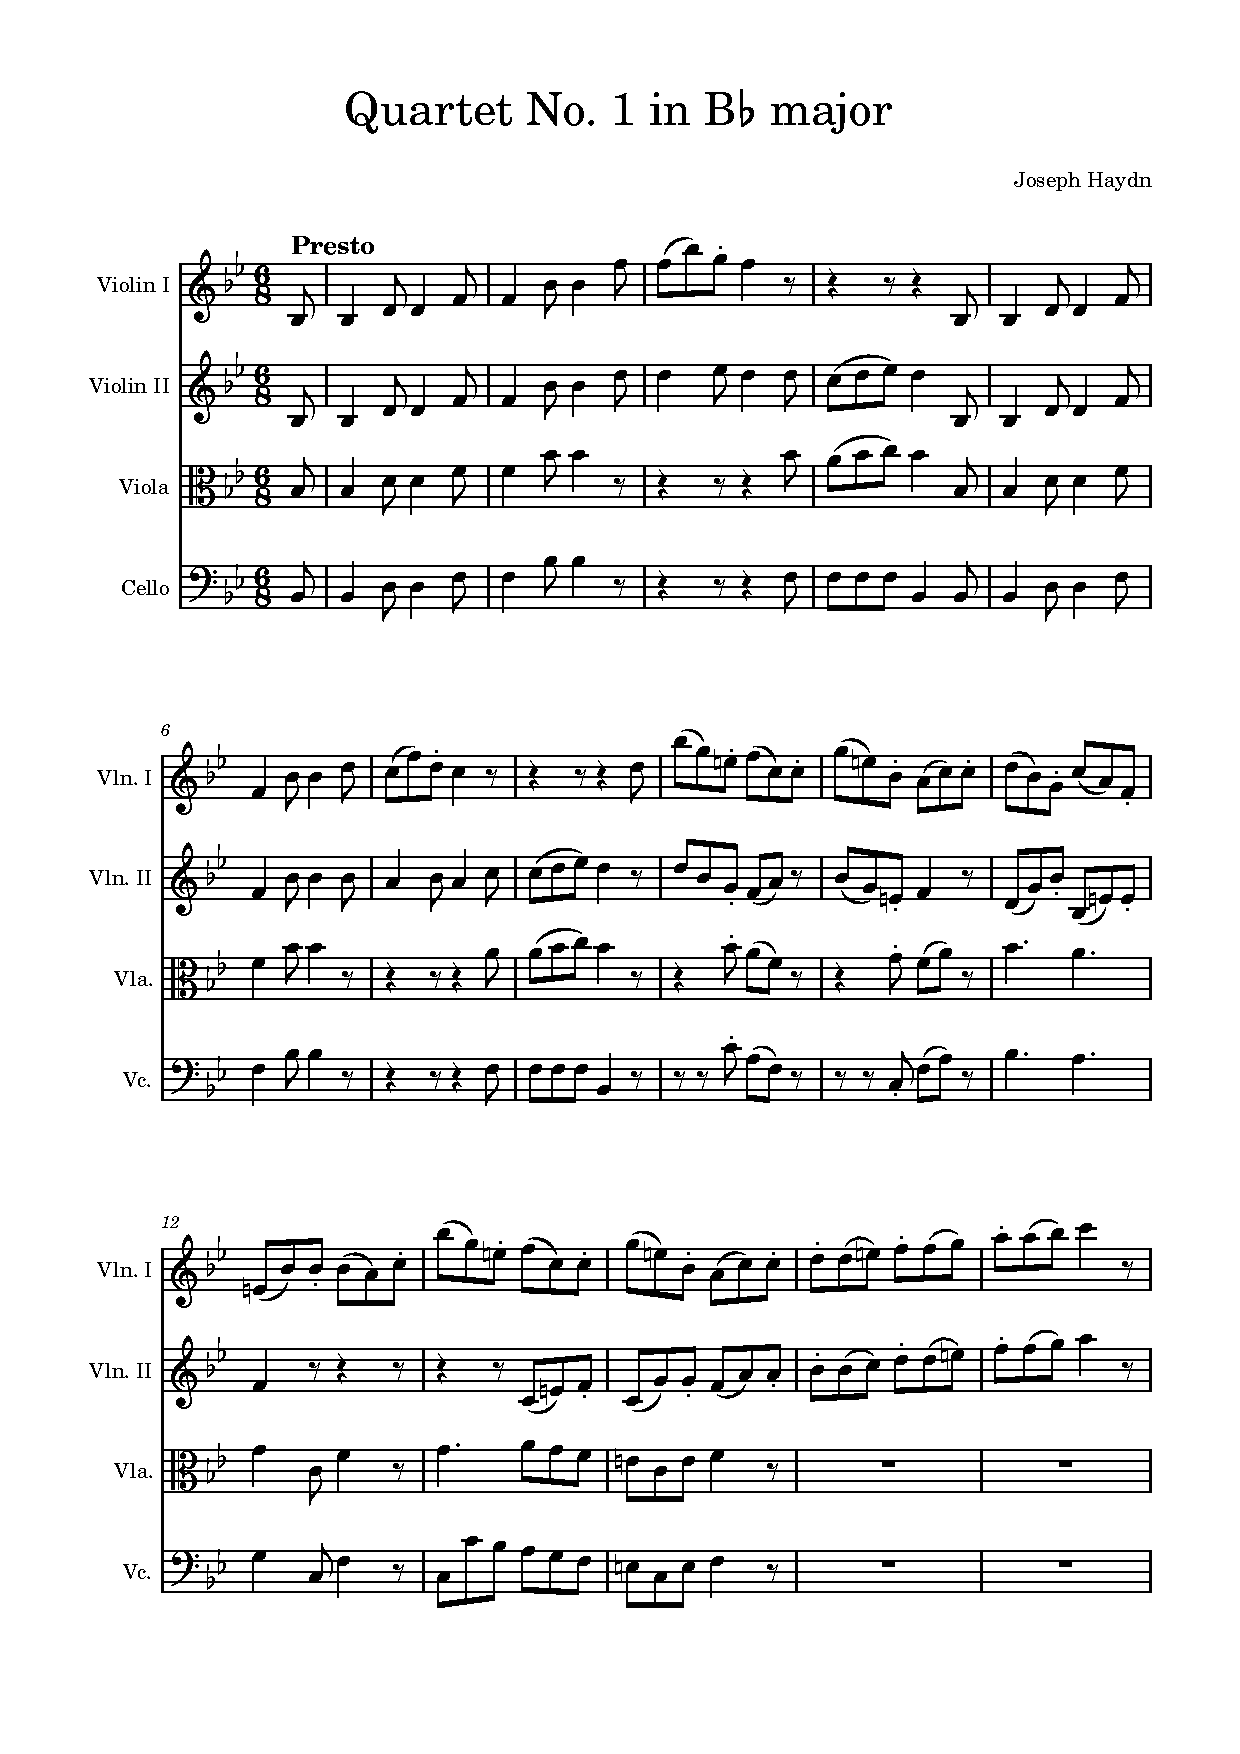
\includegraphics[width=\textwidth,page=1]{haydn-score.pdf}
    \caption{Quartet No.\ 1 in B-flat major, Op.\ 1, by Joseph Haydn, bars 1--16.}
\end{figure}

\begin{figure}
    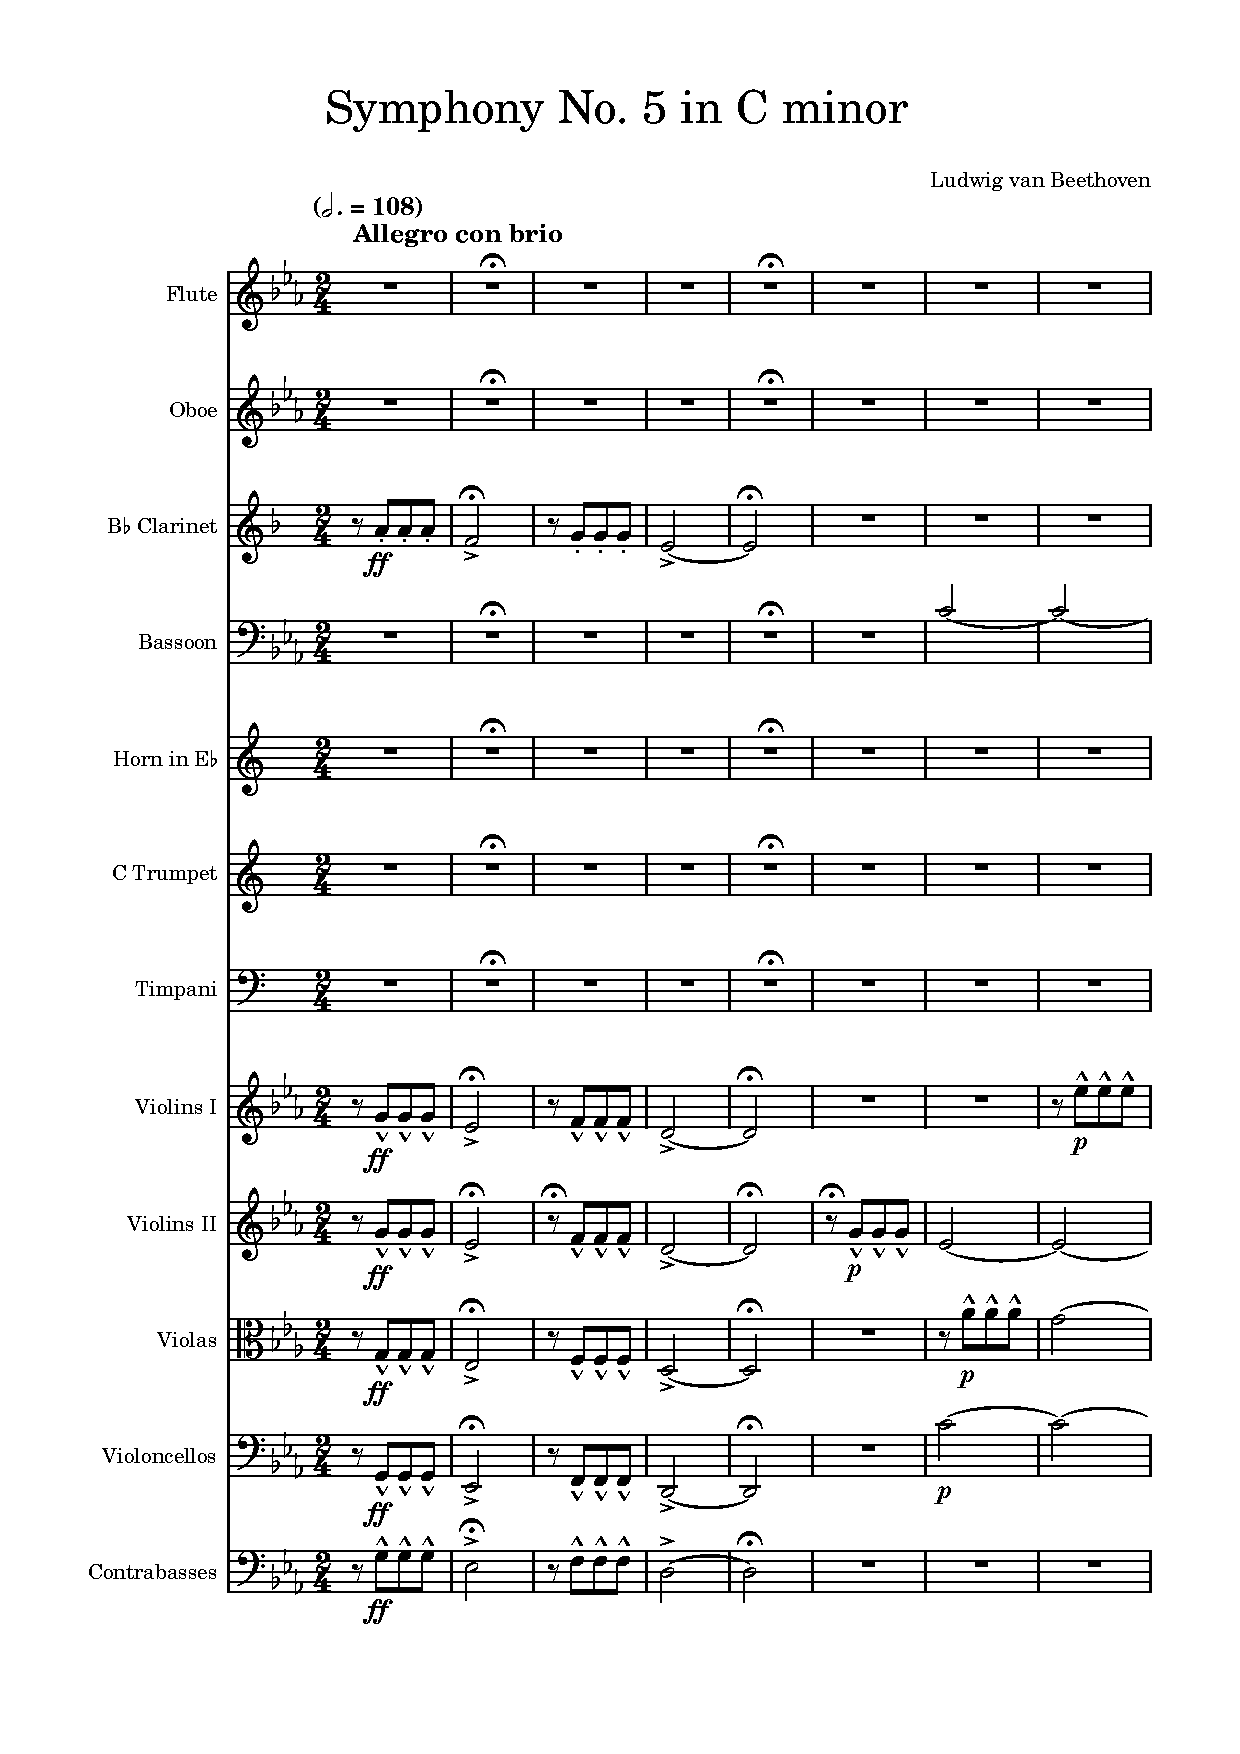
\includegraphics[width=\textwidth,page=1]{beethoven-op67.pdf}
    \caption{Symphony No.\ 5 in C minor, Op.\ 67, by Ludwig van Beethoven, bars 1--8.}
\end{figure}

Start with an undirected graph $G=(V,E)$ and a set of $n$ colours, which represent the parts for which we are arranging, with each being an independent set. Denote $x_{v,i}$ to be a binary variable such that
\begin{equation*}
    x_{v,i} =
    \begin{cases}
        1 & \text{if vertex $v$ is colour $i$} \\
        0 & \text{otherwise}
    \end{cases}
    \,,
\end{equation*}
which requires $nV$ variables. The energy is
\begin{equation*}
    H = H_A + H_B + H_C + H_D \,.
\end{equation*}

Each vertex is coloured exactly once:
\begin{equation*}
    H_A = A\sum_{v \in V}\left(1-\sum_{i=1}^{n} x_{v,i}\right)^2
\end{equation*}

Vertices of the same colour are not connected by an edge:
\begin{equation*}
    H_B = B\sum_{(u,v) \in E}\sum_{i=1}^n x_{u,i}x_{v,i}
\end{equation*}

Maximise the weighting of selected vertices:
\begin{equation*}
    H_C = -C\sum_{v \in V}\sum_{i=1}^n W_vx_{v,i}
\end{equation*}

Maximise the weighting of included edges:
\begin{equation*}
    H_D = -D\sum_{(u,v)\in E}W_{uv}\sum_{i=1}^n\sum_{j=1}^n x_{u,i}x_{v,j}
\end{equation*}

It can be seen that for $n=1$ this reduces to the MIS problem. For a score with $p$ parts, it will be impossible to colour the graph exactly with $n<p$; the parameter $A$ should be small enough to allow for some vertices to remain uncoloured. The lowest energy solutions will return coloured independent subsets of $G$ that each represents a monophonic part of the final arrangement.

\clearpage

\section*{Scientific summary for a general audience} % 200 words
\addcontentsline{toc}{section}{Scientific summary for a general audience}

The arrangement of music by hand is usually a difficult and time-consuming process, requiring a deep understanding of musical theory and structure. This study aims to automate this process via quantum computing, a technique that relies on the use of qubits, which can exist in a superposition of states. A music score can be split up into a sequence of phrases by looking at how much adjacent notes differ from each other, and turned into a graph representation with nodes and edges, where each node is a phrase, and edges between nodes mean they overlap. This graph can then be sent to a quantum computer in order to select nodes according to a set of rules that determine the properties of the arrangement. Once the nodes have been selected, the corresponding phrases can be reconstructed to create the final score. Here, an excerpt of Beethoven's String Quartet No.\ 10 is reduced to a single part, suitable for a solo instrument.

\end{document}